\chapter{Experiments}\label{C:experiments}

\section{Introduction}

All the algorithms above excluding DQN can work on continuous action spaces. This makes them suited for continuous control tasks that are common within the robotic control domain. I will conduct experiments using the Gymnasium \cite{towers2024gymnasium} library which provides a framework to use among other things some Mujoco \cite{todorov2012mujoco} environments. Specifically I will use \texttt{Ant-v5, Humanoid-v5, Pusher-v5, HalfCheetah-v5, HumanoidStandup-v5, Swimmer-v5, Hopper-v5, InvertedDoublePendulum-v5, Walker2d-v5} and \texttt{Hopper-v5} which cover a range of locomotion tasks. I will run the experiments we have looked at above on theses environments to understand how well they learn.

There are many different dimensions in which we can judge the learning performance of an algorithm. The most common and useful ones are general across not continuous control problem but all reinforcement learning problems. These common and overarching dimensions are:

\begin{itemize}
    \item Sample efficiency: How many environment interactions does it take to learn a task?
    \item Computational efficiency: How much computation does it take to learn a task?
    \item Stability: How stable is the learning process?
    \item Asymptotic performance: What is the maximum performance of the algorithm?
    \item Generalization: How well does the algorithm generalise to new tasks, be it new environments or agent?
\end{itemize}

\section{Baseline Experiments}

I will look at two things for all of my baseline algorithms. The first is the sample efficiency and the second is the computational efficiency. It is important to understand both of these metrics as it can sometimes be easier to trade computational efficiency for sample efficiency. Therefore to make a true improvment to a model it must be better at either/both of these metrics will not reducing the other metric.

\subsection{Sample Efficiency}
To measure the sample efficient I will look at the average reward over 10 episodes every 1000 steps. This will give a learning curve to demonstrate how effective its actions are given how many interactions it has had with the environments.

\begin{figure}[H]
    \centering
    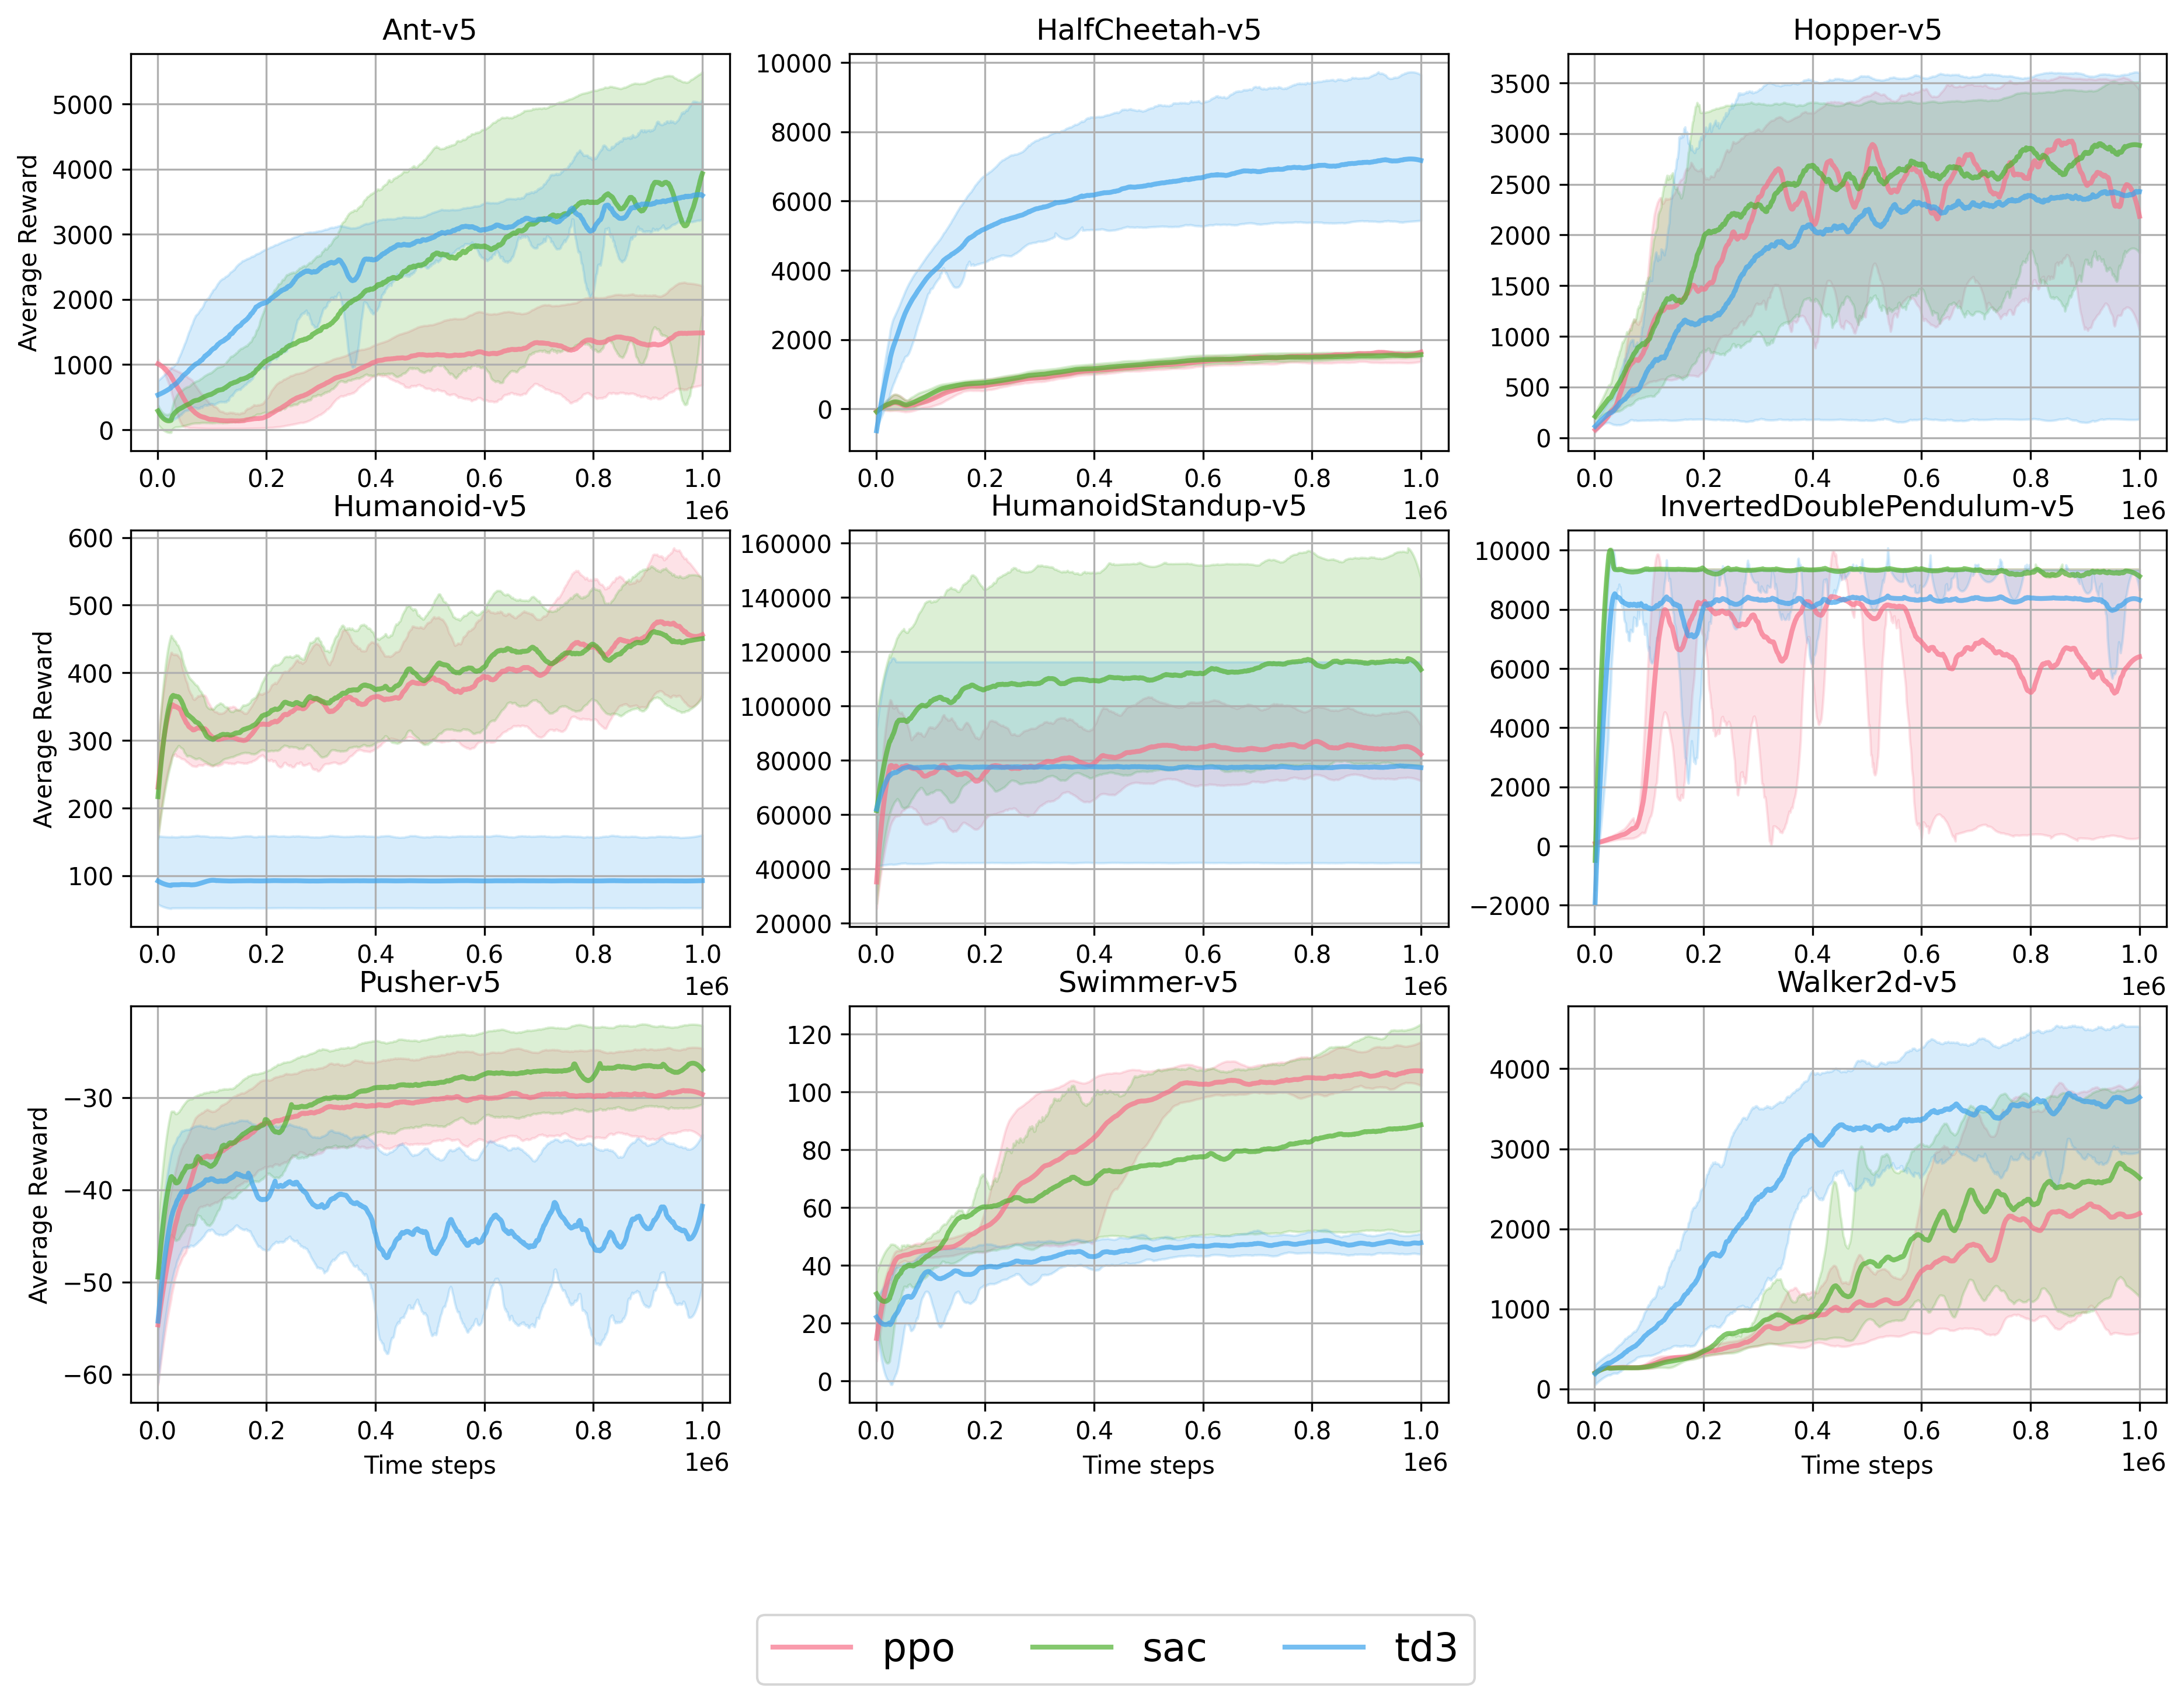
\includegraphics[width=1\textwidth]{figures/baseline_results.png}
    \caption{Sample Efficiency. The line is a smoothed average return across the 100 episodes made by each seed every 1000 times steps. The shaded area is a smoothed 70\% confidence interval highlighted }
    \label{fig:sample_efficiency}
\end{figure}

Information on the implementations of the algorithms and the hyperparameters can be found in appendix \ref{C:appendixA}. We see across the algorithms that the newer algorithms outperform the older algorithms in both sample efficiency (how steep the line is) and asymptotic performance (the maximum value of the line). It can be be seen that REDQ and TQC both outperform SAC even though they have the same foundations.

We can see that the newest algorithms are performing the best. Particularly CrossQ performs very well on the more complex environments like Humanoid and HumanoidStandup. It is also observed that CrossQ variance is a lot larger than the other algorithms which is most stark in the HumanoidStandup environment. This is likely due to the fact that CrossQ uses layer normalization which can lead to more variance in the learning process.

\textit{State how well sunrise has done.}

\dots

\subsection{Computational Efficiency}

The measure of computational efficiency is about measuring the amount of computation it takes to get a an agent to learn a certain task. As there is a variety of different algorithms the mos general method is to measure the wall clock time it takes the algorithm to complete a certain number of environment steps.

\begin{figure}[H]
    \centering
    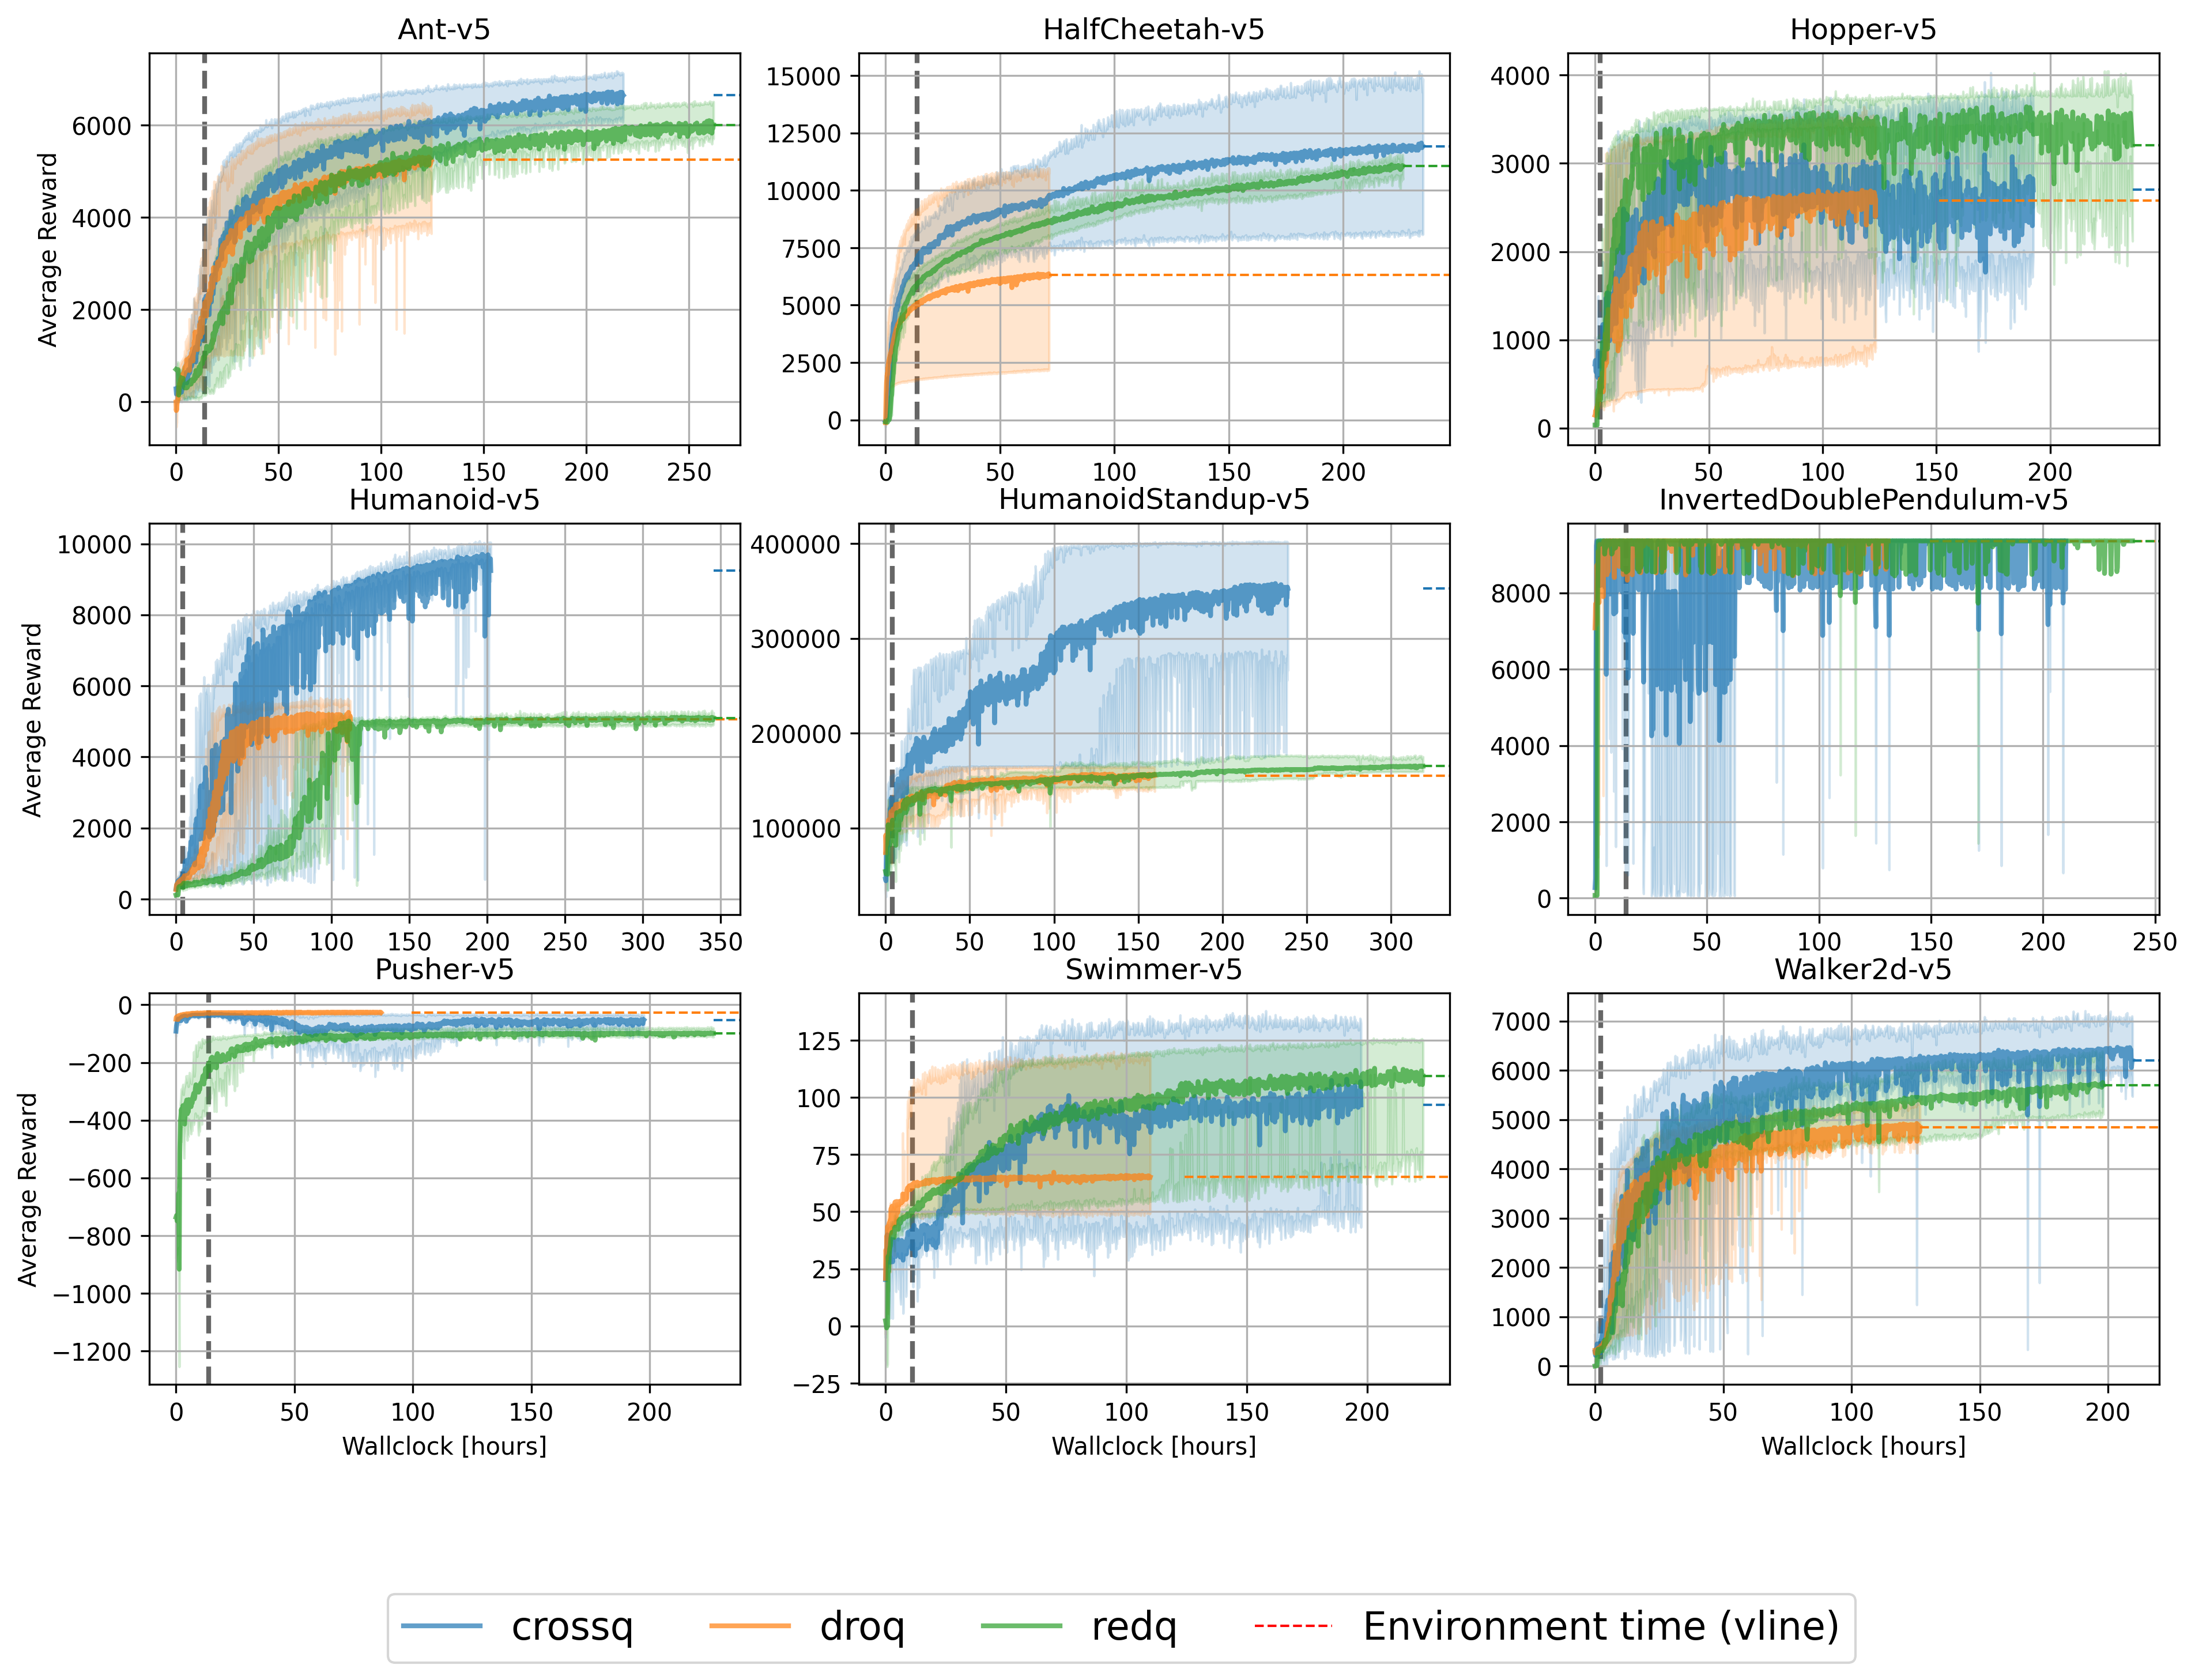
\includegraphics[width=1\textwidth]{figures/wall_clock_results.png}
    \caption{Wall clock time to get to 1 million environment time steps. Vertical lines is how long a million time-steps is in the environment. Horizontal line is the mean average reward at the end of the million steps of learning to help comparisons.}
    \label{fig:sample_efficiency}
\end{figure}

All of experiments were run on similar CPU only machines. See the appendix \ref{C:appendixA} for more information. The goal of graph is not to look at absolute time (however that is interesting to know) it is about the comparing the difference between algorithms given the same hardware.

It is interesting to note that the most modern algorithms redq and crossq are the longest running in terms of wall clock time. More importantly we can see that the method of redq having alot of critics is computationally expensive and results in a wall clock time almost 4 times that of sunrise which is also a modern ensemble method.

Looking at the horizontal lines can give us a rough idea of whether we are learning in realtime, faster than realtime or slower than realtime. We can see that for a more complicated task like HumanoidStandup we are learning significantly slower than realtime. Whereas the simpler environments are not so drastically slower than realtime. Given the hyperparameters are the same for all environments the only difference in environments is the action and state dimension as well as simulation time. Deeper analysis would have to be done to detangled the affect of simulation time and the action/state dimension in the wall clock time.

\dots

\section{Ensemble diversity}
The key idea of DSunrise is to ensure that the diversity of the ensemble of actors is maintained. As DSunrise can be directly compared to Sunrise, we can look at the diversity of the ensemble throughout training.

\begin{figure}
    \centering
    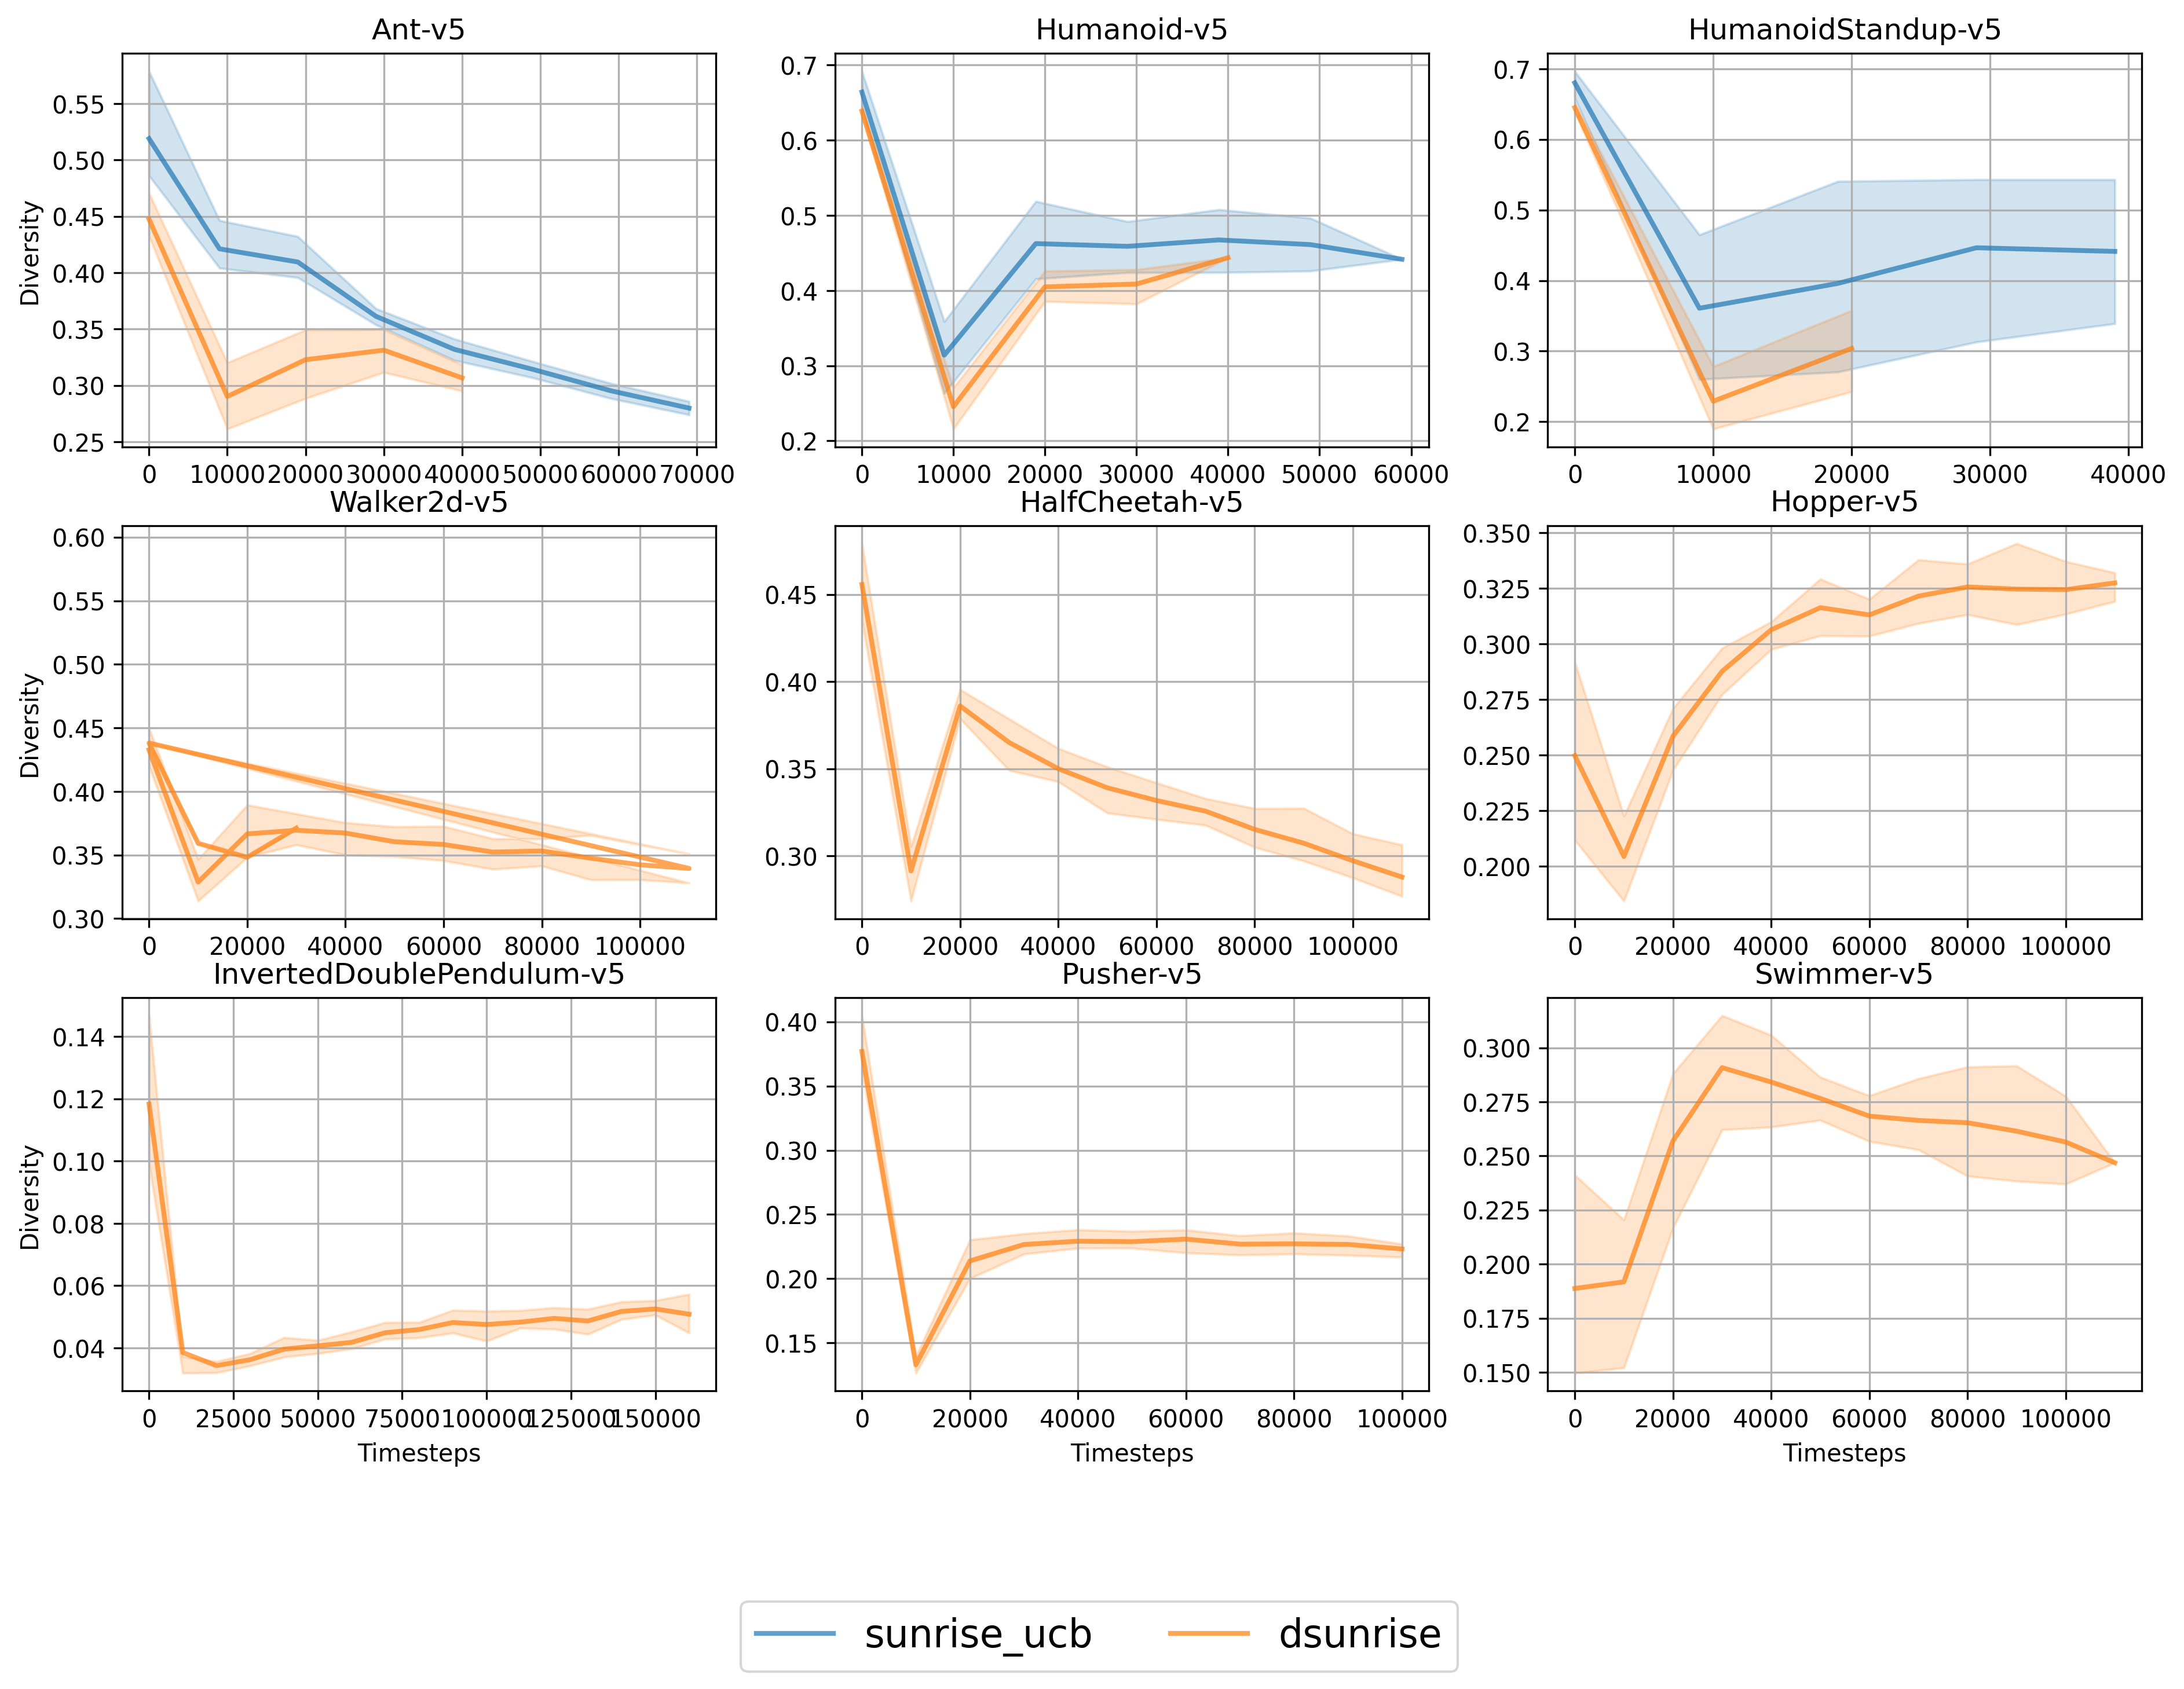
\includegraphics[width=1\textwidth]{figures/diversity_results.png}
    \caption{Diversity of the ensemble over time. The shaded area is a smoothed 70\% confidence interval highlighted.}
    \label{fig:diversity}
\end{figure}

\textit{Still waiting on the completed results for this.}

As one would expect the diversity of the ensemble decreases over time as the agents learn to do the task and converge towards the optimal policy. The goal of DSunrise is to maintain the diversity of the ensemble.